\documentclass{../../../../style/mkimain}

\series{4}
\month{květen}
\year{2023}

\begin{document}
%<*header>
\section*{IV.K Částice či vlna, to je oč tu běží}
%</header>
%úvod
V minulém seriálu jsme si odpověděli na otázku vyzařování a představili jsme si \emph{Planckův vyzařovací zákon}. 
Také jsme otevřeli téma tzv. \emph{vlnově-částicový dualismu} (světlo se může chovat jako částice a zároveň jako vlna). 
Právě zkoumání tohoto jevu se budeme věnovat v tomto seriálu.

Náš příběh začíná na začátku 20. století  u 26letého Alberta Einsteina, který se v té době mimo jiné pokoušel vysvětlit tzv. \emph{fotoelektrický jev}.

Fotoelektrický jev (\emph{fotoefekt}) spočívá v uvolnění (a následné emitaci) elektronů z obalu atomů po 
absorpci \emph{elektromagnetického záření} (světla) danou látkou. Podle klasické fyziky by měla energie odlétajících elektronů záviset na \emph{intenzitě} záření, ale experimentálně 
se dokázalo, že jejich energie záleží hlavně na frekvenci zdroje. K vysvětlení této závislosti použil Einstein roku 1905 Planckovu myšlenku \emph{kvantování} a přisoudil tak 
elektronům energii kvanta elektromagnetického záření, tedy fotonu, $E=h\nu$, kde $h$ je \emph{Planckova konstanta} a $\nu$ je \emph{frekvence elektromagnetického záření}. Toto vysvětlení spolu s 
Planckovým vyzařovacím zákonem stálo u zrodu kvantové fyziky a změnilo doposud čistě vlnový pohled klasické fyziky na světlo.

O několik let později se na začátku 20. let 19. století mladý \emph{Louis de Broglie} zamýšlel nad tím, jestli by nešlo tuto úvahu zobecnit. Snažil se tedy přiřadit 
částicím jako např. eletronům a protonům \emph{vlnový charakter}. Ve své doktorské práci roku 1924 přišel s následujím vztahem mezi vlnovou délkou a rychlostí částice.
$$
\lambda=\frac{h}{p}\text{,}
$$
kde $\lambda$ je tzv. \emph{de Broglieho vlnová délka}\footnote{V některých publikacích můžete najít i termín \emph{de Broglieova} vlnová délka}, $p$ je hybnost 
částice, $h$ je již několikrát zmiňovaná Planckova konstanta.

Tyto myšlenky byly následně ověřeny tzv. \emph{dvojštěrbinovým experimentem}. Při provedení experimentu se zdrojem elektronů (viz obr.1) byl na 
detektoru pozorován interferenční obrazec podobný tomu, který vznikl při měření se zdrojem světla (viz obr.2). Tato skutečnost dokazuje, že i elektrony se mohou chovat jako vlny.

\begin{figure}[H]
    \minipage{0.42\textwidth}
      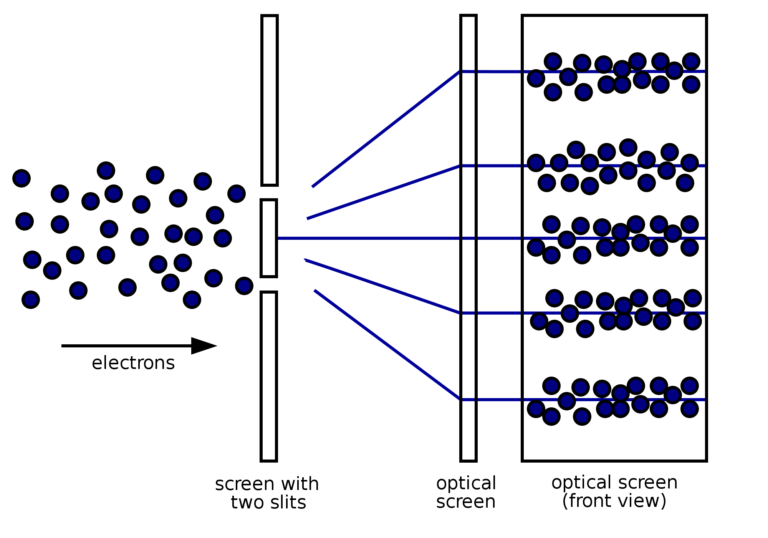
\includegraphics[width=\linewidth]{double-slit-exp.png}
      \begin{center}
        Obr.1: Schéma dvojštěrbinového experimentu s elektronovým paprskem
        \end{center}
    \endminipage\hfill
    \minipage{0.42\textwidth}
      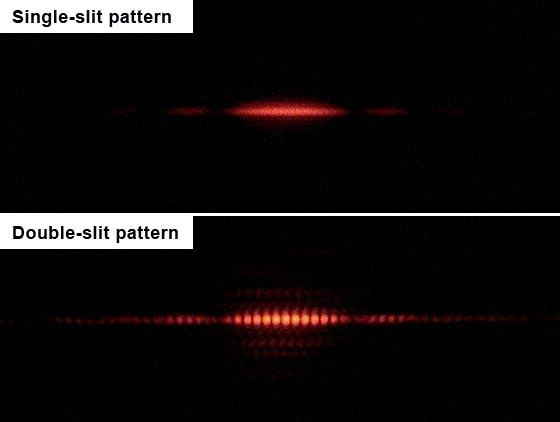
\includegraphics[width=\linewidth]{double-slit-difraction.jpg}
      \begin{center}
        Obr.2: Pozorovaný interferenční obrazec
        \end{center}
    \endminipage
  \end{figure}
\noindent\textbf{Úloha:}

%<*task>

%\begin{enumerate}[\noindent {}]
%\item otazka
%  \begin{choices}
%    \choice
%  \end{choices}
%\end{enumerate}

%</task>
\end{document}


% doktorská práce (brokolice) - obecná formulace dualismu (vlna -> částice --> částice -> vlna)

% btw 2 || exp. -> důkaz (za jistých podmínek - pozorování)

%       |     )  )  ))         |
%   / - -) ) ) ) ) ))))        |
% -     |  ## # ) ) )          |
%   \ - -) ) ) ) ) ) ) )       |
%       |     )) ) )))         |

% DeBroglieho vlna? ANO (určitě)
% $$ - možná na začátek
% \lambda=\frac{h}{p}
% $$

% 

% Bohrův model -> seriál: Schrödingerův model atomu

% !!! footnote odkaz na výfučtení 5. série 12. ročník !!!
%\footnote{Pokud si od nás chcete na toto téma přečíst víc: \url!vyfuk.org/_media/ulohy/r12/s5/vyfucteni5.pdf!}

